\section{Accuracy}
\label{sec:accuracy}
 
One of the most reliable way to assess the simulation's accuracy at evolving particles
is to measure the density power spectrum at late time, and compare to non-linear prediction. 
For an over-density field $\delta({\bf \it x})$, the power spectrum is extracted from the two point function in Fourier space as:
\begin{eqnarray}
\langle | \delta ({\bf \it k}) \delta ({\bf \it k'}) | \rangle = (2\pi)^{3}P(k)\delta_{D}({\bf \it k'} - {\bf \it k})
\label{eq:power}
\end{eqnarray}
where the angle bracket corresponds to an ensemble (or volume) average.
We plot in Fig. \ref{fig:power_highres} the dimensionless power spectrum in a RANGER4000 simulation and
observe that the agreement with the non-linear prediction of \cite{Lewis:1999bs} is at the per cent level over a large dynamical range.
The drop of power at high-$k$ is caused by the finite resolution, and the fluctuations at low-$k$ are caused by the white noise imposed
in the initial conditions. 

\begin{figure*}%[ht]
  \begin{center}
    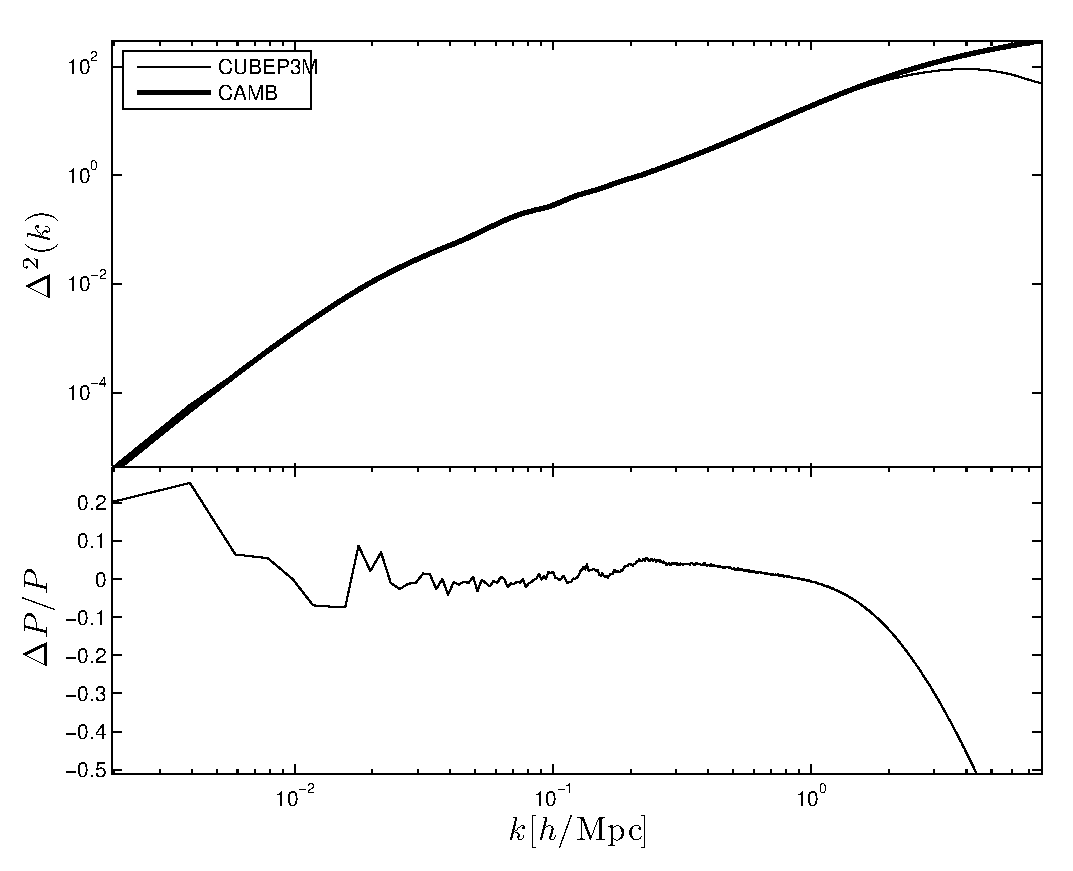
\includegraphics[width=5.2in]{graphs/power_highres.eps}
  \caption{Dark matter power spectrum, measured at $z=0$ in a RANGER4000 simulation.
    \label{fig:power_highres}}
\end{center}
\end{figure*}

The actual force of gravity in the p$^3$m algorithm,
as felt by a single particle, is presented in Fig. \ref{fig:den_force_ppext0}.
This shows the force versus distance -- in fine cell units -- a calculation that was performed in a CITA256 realization in two steps: 
1- we compute the force on each particle in a given distribution, as done at every time step.
2- we remove a selected particle, compute the force again on all particles, and record on a file the 
force difference (before  and after the removal) as a function of the distance to the `hole'.

Particles in the same fine cell follow the exact $1/r^{2}$ curve. The scatter at 
  distances of the order of the fine grid is caused by the NGP interpolation scheme:
  Particles in adjacent fine cells can be actually very close, as seen in the upper left region of this plot,
  but feel the mesh force at grid cell distances,
  creating up to an order of magnitude loss in the force.
As the separation approaches a tenth of the box size or so, the force on the coarse mesh deviates
from Newton's law in order to preserve periodic boundary conditions. 
This feature, however, can be turned off at compilation time.


Fig. \ref{fig:den_force_fracErr} shows the fractional error on the force along the radial and tangential directions.
It is larger than in {\small PMFAST} at grid scales, largely due to the fact that the fine mesh force is performed with an NGP interpolation scheme -- as opposed to CIC -- which shows a larger scatter about the theoretical value. 
As discuss in the next section, to minimize this effect, we apply a random offset to all the particles,
such that this undesired scatter is average out over a few time steps.



\begin{figure}%[ht]
  \begin{center}
    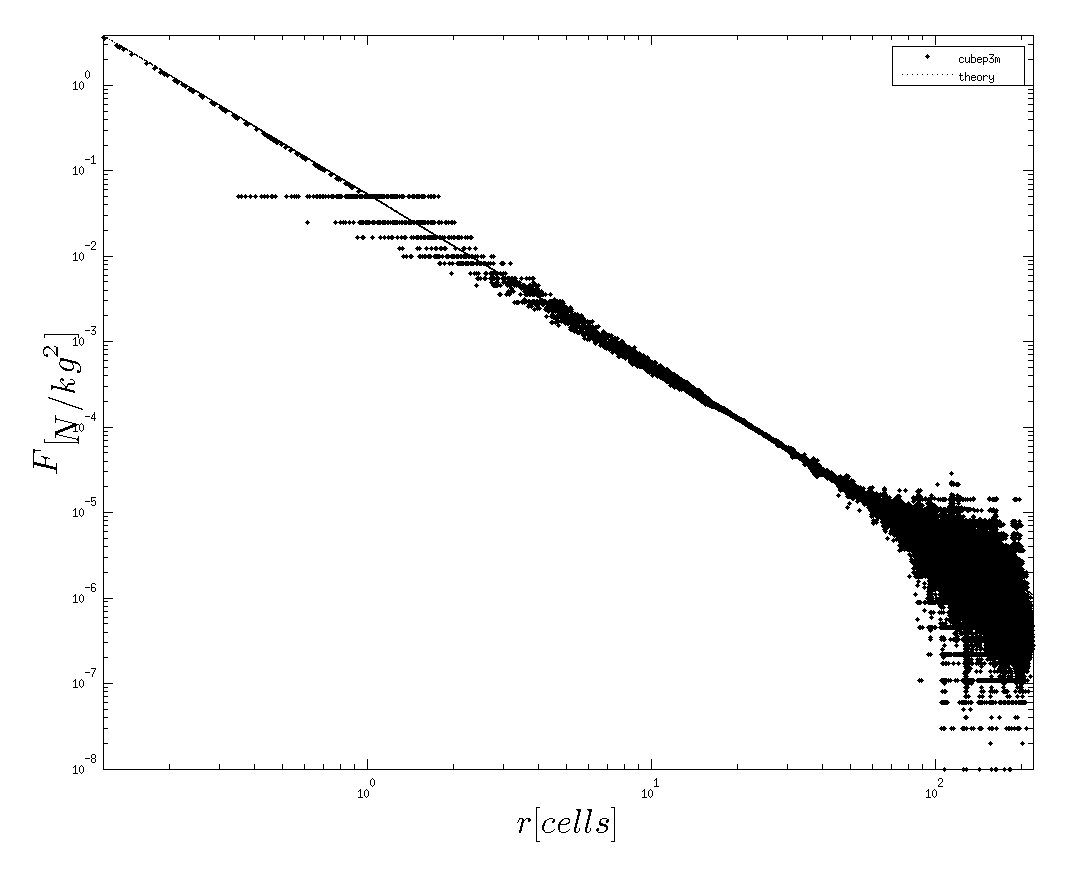
\includegraphics[width=3.2in]{graphs/densityForce_ppext=0.eps}
  \caption{Gravity force in of the p$^3$m algorithm, versus distance in fine mesh cell units, compared with the exact $1/r^{2}$ law.
    This particular calculation was obtained in a CITA256 realization. 
    \label{fig:den_force_ppext0}}
\end{center}
\end{figure}

\begin{figure}%[ht]
  \begin{center}
    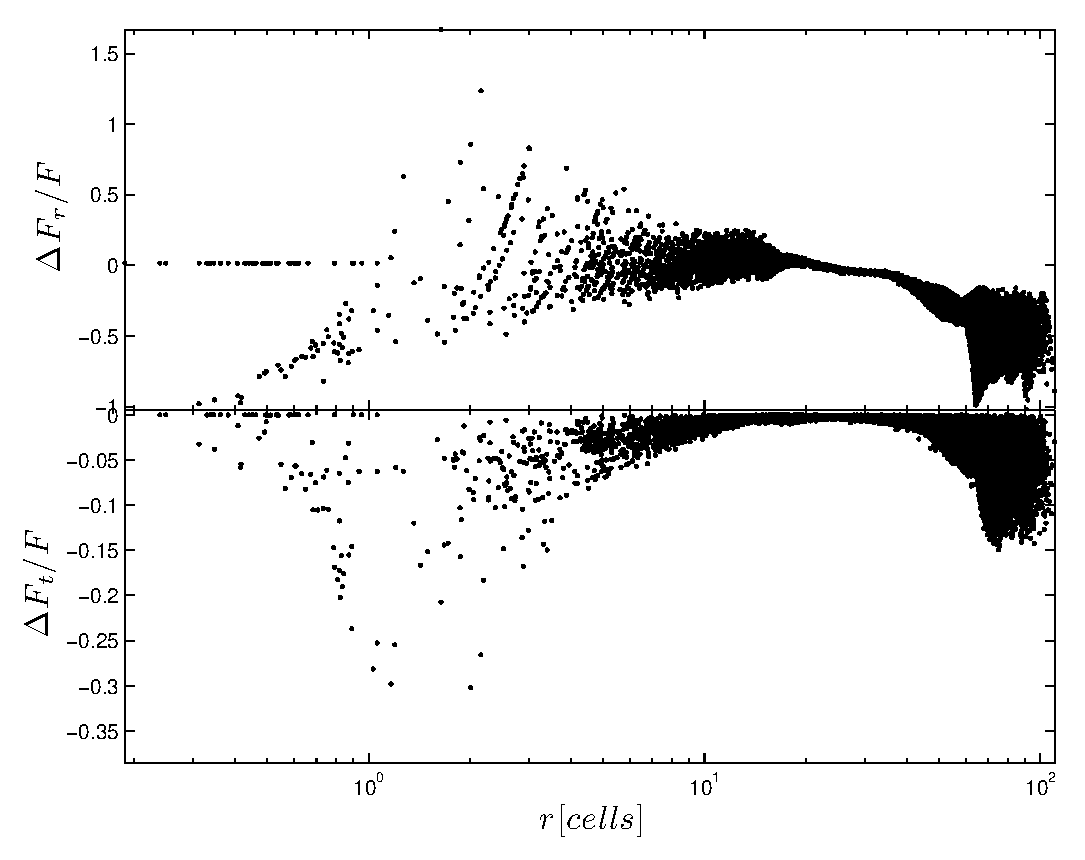
\includegraphics[width=3.2in]{graphs/densityForce_fracErr.eps}
  \caption{Fractional error on the force in of the p$^3$m algorithm, in the radial (top) and tangential(bottom) directions.
    \label{fig:den_force_fracErr}}
\end{center}
\end{figure}


\section{Systematics}
\label{sec:systematics}

\subsection{Mesh force at grid distances}

The biggest problem with the straightforward pp force calculation is that the results 
are anisotropic and depend on the location of the fine mesh with respect 
to the particles. As an example, consider two particles on either side of a grid 
cell boundary, experiencing their mutual gravity attraction via the (NGP) mesh force with a 1-grid cell separation.
 If, instead, the mesh was shifted such that they were
within the same cell, they would experience the (larger) pp force. 
This effect is especially pronounced at the early stages of the simulation where
the density is more homogeneous, and leads to mesh artefacts appearing
in the density field. In order to minimize this systematic effect, 
we randomly shift the particle distribution relative to the mesh by a small
amount -- up to 2 fine grid cells in magnitude -- in each
dimension and at each time step.  This adds negligible computational
overhead as it is applied during the particle position update,
and suppresses the mesh behaviour that otherwise grows over multiple time steps.
It is possible to shift back the particles at the end of each time steps,
which prevents a random drift of the whole population, a necessary step 
if one needs to correlate the initial and final positions of the particles for instance,
or for hybrid dark matter -- MHD simulations.
 
We ensure that, on average, this solution balances out the mesh feature,
by tuning the force kernels such as to provide  force as evenly balanced as possible at grid cell distances
and at the cutoff length ($r_{c}=16$ fine cells).
These adjustments are performed from the pairwise force test described in section \ref{sec:accuracy}.
We note that this is one of the driving argument to extend the pp force outside the fine mesh cell,
since the scattering of the NGP force about the actual $1/r^{2}$ law drops rapidly as the distance increases.
As discussed in section \ref{subsec:extendedpp}, this gain in accuracy comes at a price,
a choice that  must be carefully balanced.

We present in Fig. \ref{fig:disp_mesh} the dramatic impact of removing the random offset in the code.
The power spectrum is completely wrong, caused by the large scatter in the force on the fine mesh.
In this scatter is not averaged over, the error directly adds up at each time step. {\small PMFAST}
did not have this problem since it used CIC interpolation on both meshes.  
This test was performed with CITA128 simulations of very large box size,
which should in principle agree with linear predictions up to the resolution.
The output redshifts are very early, and the upper most curve ($z=10$) was obtained after
about 60 timesteps.
We see that deviations are enormous when the random offset is turned off.

\begin{figure}%[ht]
  \begin{center}
    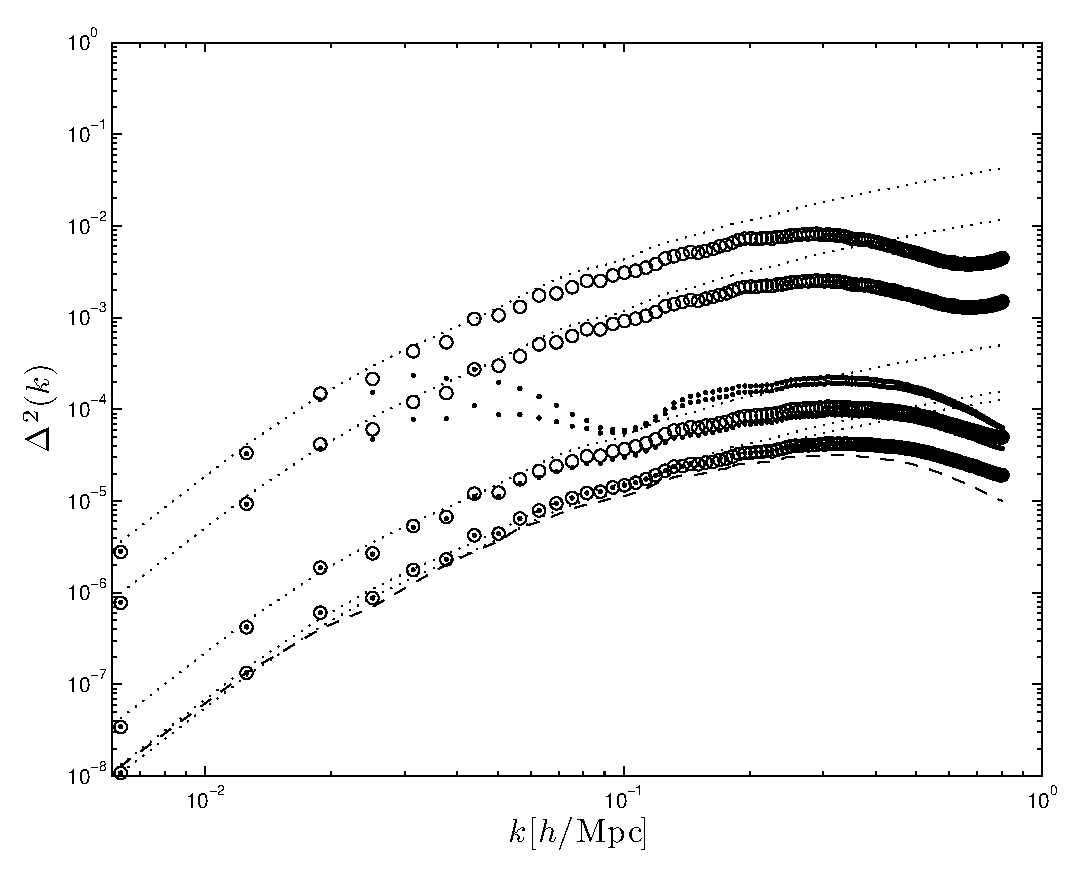
\includegraphics[width=3.2in]{graphs/power_w_wo_disp_mesh.eps}
  \caption{Dark matter power spectrum, measured at $z=180$, $100$, $20$ and $10$, in a series of CITA128 realizations that are 1000 Mpc/$h$ per side. The dashed line represent the initial condition power spectrum, the dotted lines are the linear predictions, and  the open circles the standard p$^3$m configuration. 
  The dots were obtained by simply removing the random particle offset that is usually applied at each time step. \label{fig:disp_mesh}}
\end{center}
\end{figure}


\subsection{Constraining redshift jumps}

At early stages of the simulation, the density fields is rather homogenous, causing the force of gravity to be
rather weak everywhere. In that case, the size of the redshift jumps is controlled by a limit in the cosmological expansion.
If the expansion jump is too large, the size of the residual errors can become significant, and one can observe, for instance,
a growth of structure that does not match the predictions of  linear theory even at the largest scales.
One therefore needs to choose a maximum step size. In {\small CUBEP3M}, this is controlled by $r_{max}$, which is the fractional step size,
$\mbox{d}a/(a + \mbox{d}a)$ and is set to $0.05$ by default.  Generally, a simulation should start at a redshift high enough that
the initial dimensionless power spectrum is well under unity at all scales. This ensures that the Zel'dovich approximation
 holds at the per cent level at least. A drop of accuracy can occur if one starts the simulation too early, where
 truncation error will be significant at the early time steps.


It is possible to reduce this effect, and thereby improve significantly 
the accuracy of the code, by modifying the value of $r_{max}$, at the cost of increasing the total number of time steps.
Fig. \ref{fig:ra_max} shows a comparison of late time power spectra of a series of CITA256 realizations that originate from the same initial conditions, 
and used the same random seeds to control the fine mesh shifts (mentioned above): only the value of $r_{max}$ was modified between each run. 
We observe that the impact is mostly located in the non-linear regime, where decreasing the time step to 0.006 
allows the simulation to recover about 30 per cent of dimensionless power at the turn over scale, in this simulation configuration.
This gain is greatly affected by the choice of initial redshift, the resolution, and the box size, and ideally one would make
test runs in order to optimize a given configuration.  
As expected, the {\small CPU} resources required to run these simulations increase rapidly as $r_{max}$ decreases, as seen in Table \ref{table:ra_max}. 
In this test case, reducing further at 0.001 shows only a mild improvement in accuracy, but the increase in time is more than a factor of four.


\begin{figure}%[ht]
  \begin{center}
    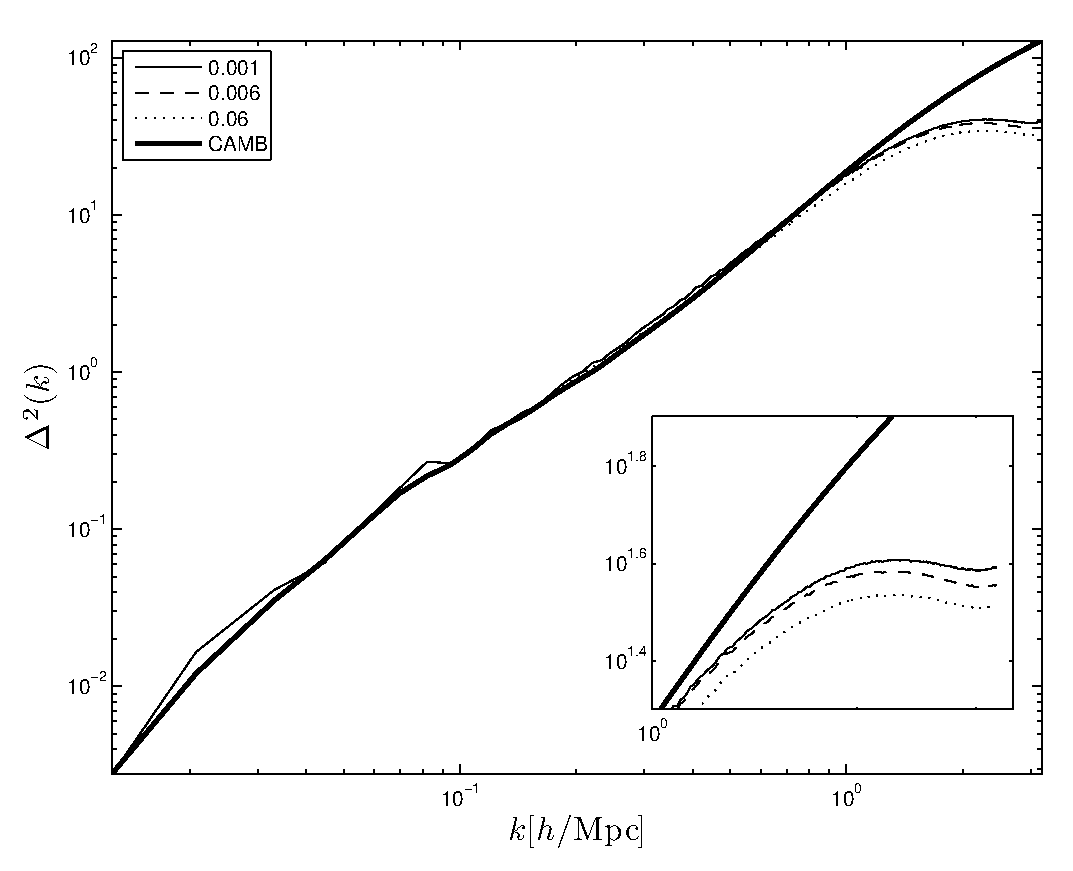
\includegraphics[width=3.2in]{graphs/power_ra_max.eps}
  \caption{Dark matter power spectrum, measured at $z=0$ in a series of CITA256 realizations. 
 The starting redshift ofwas raised to $z=200$ to enhance the systematic effect. The different curves show different values of $r_{max}$. 
  The resources required to run these simulations increase rapidly as $r_{max}$ decreases, as seen in Table \ref{table:ra_max}.    \label{fig:ra_max}}
\end{center}
\end{figure}

\begin{table}
\begin{center}
\caption{Scaling in {\small CPU} resources as a function of the value of $r_{max}$. The tests were performed 
on the CITA Sunnyvale cluster, and general trends could vary slightly on other machines.}
\begin{tabular}{|l|c|c|}
\hline 
$r_{max}$         & time (h)   \\                 
\hline
 $0.1$ & 1.46 \\
 $0.06$ & 1.48\\
 $0.01$ & 1.67 \\
 $0.006$ & 1.91\\
 $0.003$ & 2.83 \\
 $0.002$ & 4.13\\
 $0.001$ & 8.15\\
\hline
\end{tabular}
\label{table:ra_max}
\end{center}
\end{table}


{\bf (Any other systematics effects we want to discuss here?)}

 


